\documentclass[aspectratio=169,10pt]{beamer}
\usetheme{metropolis}
\usepackage{listings}
\usepackage{tikz}
\usepackage{amsmath,amssymb}
\usepackage{xcolor}
\usepackage{stmaryrd}
\usepackage{mathtools}

% Compact beamer spacing
\setbeamertemplate{frametitle}{\vspace{-0.2em}\insertframetitle\vspace{-0.3em}}
\setbeamersize{text margin left=6mm, text margin right=6mm}
\usetikzlibrary{arrows.meta, positioning, calc, decorations.pathreplacing, shapes.geometric}

% Colors
\definecolor{siteA}{HTML}{4C72B0}
\definecolor{siteB}{HTML}{DD8452}
\definecolor{siteC}{HTML}{55A868}
\definecolor{conflict}{HTML}{C44E52}
\definecolor{ok}{HTML}{55A868}
\definecolor{codebg}{HTML}{F5F5F5}
\definecolor{tradbox}{HTML}{FFF3E0}
\definecolor{sheafbox}{HTML}{E8F5E9}
\definecolor{keyblue}{HTML}{1565C0}

\lstset{
  basicstyle=\ttfamily\tiny,
  backgroundcolor=\color{codebg},
  frame=single,
  framerule=0pt,
  columns=fullflexible,
  keepspaces=true,
  escapeinside={(*}{*)},
  keywordstyle=\color{siteA}\bfseries,
  stringstyle=\color{siteB},
  commentstyle=\color{gray}\itshape,
  language=Python,
  morekeywords={deppy,requires,guarantee},
  showstringspaces=false,
  aboveskip=4pt,
  belowskip=2pt,
}

\newcommand{\Sem}{\mathcal{F}}
\newcommand{\Cat}{\mathbf{S}}
\newcommand{\Poset}{\mathbf{Poset}}
\newcommand{\op}{\mathrm{op}}

% Key insight box
\newcommand{\keyinsight}[1]{%
  \vspace{2pt}
  \begin{center}
  \colorbox{sheafbox}{\parbox{0.88\textwidth}{\centering\small\textbf{\textcolor{keyblue}{Key insight:}} #1}}
  \end{center}
  \vspace{-4pt}
}

\title{\textbf{DepPy}: Sheaf-Descent Semantic Typing for Python}
\subtitle{One framework for type checking, equivalence, and bug finding}
\author{Halley Young}
\date{}

\begin{document}

% ══════════════════════════════════════════════════════════════════════════════
\begin{frame}[plain]
\vfill
{\Large\bfseries DepPy: Sheaf-Descent Semantic Typing for Python}

\vspace{0.5em}
{\normalsize One framework for type checking, equivalence, and bug finding}

\vspace{1em}
{\normalsize Halley Young}
\vfill
\end{frame}

% ══════════════════════════════════════════════════════════════════════════════
% SLIDE 1 — The Problem (~1.5 min)
% ══════════════════════════════════════════════════════════════════════════════
\begin{frame}{The Problem: Local Facts, Global Conclusions}

Every program analysis does the same thing:

\begin{enumerate}
  \item Collect \textbf{local facts} at program points
        {\small (types, invariants, pre/post-conditions)}
  \item \textbf{Compose} them into a global conclusion
        {\small (whole-program typing, correctness proof, bug report)}
  \item Report where composition \textbf{fails}
        {\small (type errors, counterexamples, alarms)}
\end{enumerate}

\vspace{0.3em}
\textbf{The catch:} every tool re-invents composition from scratch.

{\small
\begin{tabular}{@{}ll@{}}
Abstract interpretation & fixed-point iteration + widening \\
Type checking & structural induction over typing rules \\
Hoare logic & weakest precondition / sequential composition \\
Model checking & reachability over product automaton \\
\end{tabular}
}

\keyinsight{Sheaf theory \emph{is} the mathematics of local-to-global composition.
One framework, one soundness proof, all analyses.}

\end{frame}

% ══════════════════════════════════════════════════════════════════════════════
% SLIDE 2 — The Setup (~2 min)
% ══════════════════════════════════════════════════════════════════════════════
\begin{frame}{Programs as Sheaves: The Three Ingredients}

\begin{columns}[T]
\column{0.52\textwidth}

\textbf{1.\ Sites} — observation points in a program

{\small A category $\Cat$ whose objects are program points
(argument boundaries, branch guards, return sites, SSA values, \ldots)
and morphisms are data-/control-flow edges.
DepPy defines \textbf{14 site families} (\texttt{SiteKind}).}

\vspace{0.3em}
\textbf{2.\ Sections} — type facts at each site

{\small A \emph{presheaf} $\Sem : \Cat^{\op} \to \Poset$ assigns a poset of facts
to each site, with \emph{restriction maps} along edges.
Each section carries: carrier type, refinements,
trust level, provenance, witnesses.}

\column{0.44\textwidth}

\textbf{3.\ Covers} — when do sites ``see everything''?

{\small A \emph{Grothendieck topology} $J$ declares which site families
$\{U_i \to U\}$ \emph{cover} $U$, via three axioms:}
{\small
\begin{itemize}
  \item \textbf{Identity}: self-cover
  \item \textbf{Stability}: pullback preserves covers
        {\scriptsize (specialization is free)}
  \item \textbf{Transitivity}: refining covers compose
        {\scriptsize (modular analysis for free)}
\end{itemize}
}

\begin{center}
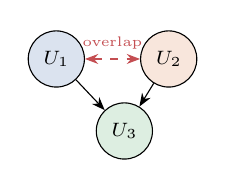
\begin{tikzpicture}[>=Stealth, font=\scriptsize, node distance=0.6cm]
  \node[circle, draw, fill=siteA!20, minimum size=0.45cm] (a) {$U_1$};
  \node[circle, draw, fill=siteB!20, minimum size=0.45cm, right=0.7cm of a] (b) {$U_2$};
  \node[circle, draw, fill=siteC!20, minimum size=0.45cm, below right=0.4cm and 0.35cm of a] (c) {$U_3$};
  \draw[->] (a) -- (c);
  \draw[->] (b) -- (c);
  \draw[<->, dashed, conflict] (a) -- node[above, font=\tiny] {overlap} (b);
\end{tikzpicture}
\end{center}

\end{columns}

\end{frame}

% ══════════════════════════════════════════════════════════════════════════════
% SLIDE 3 — The Sheaf Condition (~2 min)
% ══════════════════════════════════════════════════════════════════════════════
\begin{frame}{The Sheaf Condition: Local $\to$ Global}

Given a cover $\{U_i\}$ and a local section $\sigma_i \in \Sem(U_i)$ at each site:

\vspace{0.2em}
\begin{center}
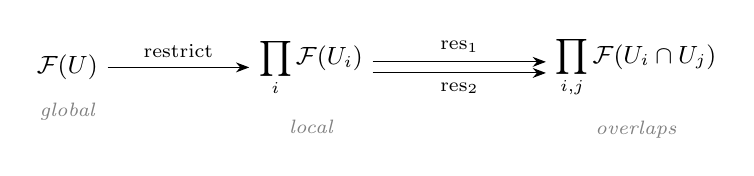
\begin{tikzpicture}[>=Stealth, node distance=1.4cm, font=\small]
  \node (FU) {$\Sem(U)$};
  \node[right=1.8cm of FU] (prod) {$\displaystyle\prod_i \Sem(U_i)$};
  \node[right=2.2cm of prod] (coprod) {$\displaystyle\prod_{i,j} \Sem(U_i \cap U_j)$};
  \draw[->] (FU) -- node[above, font=\scriptsize] {restrict} (prod);
  \draw[->, transform canvas={yshift=2pt}] (prod) -- node[above, font=\scriptsize] {$\mathrm{res}_1$} (coprod);
  \draw[->, transform canvas={yshift=-2pt}] (prod) -- node[below, font=\scriptsize] {$\mathrm{res}_2$} (coprod);
  \node[below=0.05cm of FU, font=\scriptsize\itshape, text=gray] {global};
  \node[below=0.05cm of prod, font=\scriptsize\itshape, text=gray] {local};
  \node[below=0.05cm of coprod, font=\scriptsize\itshape, text=gray] {overlaps};
\end{tikzpicture}
\end{center}

\vspace{0.1em}
{\small
\textbf{Sheaf condition} (implemented in \texttt{SheafConditionChecker}):
\begin{enumerate}
  \item \textbf{Agreement}: on every overlap $U_i \cap U_j$, the restricted
        sections agree: $\sigma_i|_{U_i \cap U_j} = \sigma_j|_{U_i \cap U_j}$
  \item \textbf{Gluing}: if all overlaps agree, there exists a \emph{global section}
        $\sigma \in \Sem(U)$ that restricts to each $\sigma_i$
  \item \textbf{Uniqueness}: the global section is unique
\end{enumerate}
}

\keyinsight{Agreement $\Rightarrow$ sound composition.
Failure to agree $\Rightarrow$ a \emph{cocycle} $[\alpha] \in H^1$
that \textbf{names the exact pair of sites} where things go wrong.}

\end{frame}

% ══════════════════════════════════════════════════════════════════════════════
% SLIDE 4 — Cohomological Errors (~1.5 min)
% ══════════════════════════════════════════════════════════════════════════════
\begin{frame}{When Gluing Fails: Cohomological Bug Classification}

\v{C}ech cohomology grades the obstruction:

\vspace{0.2em}
{\small
\begin{tabular}{@{}lll@{}}
\textbf{Degree} & \textbf{Mathematical meaning} & \textbf{PL meaning} \\
\hline
$H^0(\mathcal{U}, \Sem)$ & Global sections & Consistent whole-program typing \\
$H^1(\mathcal{U}, \Sem)$ & Gluing obstructions & \textbf{Type errors / bugs} \\
$H^2(\mathcal{U}, \Sem)$ & Higher obstructions & Higher-order inconsistencies \\
\end{tabular}
}

\vspace{0.3em}
\begin{columns}[T]
\column{0.45\textwidth}
\colorbox{tradbox}{\parbox{0.9\textwidth}{\small
\textbf{Traditional:}\\
``Line 42: expected \texttt{int}, got \texttt{str}''\\[2pt]
\emph{One location; root cause elsewhere.}
}}

\column{0.45\textwidth}
\colorbox{sheafbox}{\parbox{0.9\textwidth}{\small
\textbf{Sheaf obstruction:}\\
``Overlap of $U_3, U_7$: \texttt{int} vs \texttt{str}''\\[2pt]
\emph{Names both sites + witness.}
}}
\end{columns}

\vspace{0.2em}
{\small DepPy's \texttt{ObstructionData}: cohomology class + conflicting overlaps + explanation.
Trivial $H^1$ = fix one section. Non-trivial = genuine conflict.}

\end{frame}

% ══════════════════════════════════════════════════════════════════════════════
% SLIDE 5 — Connection to Familiar PL (~1.5 min)
% ══════════════════════════════════════════════════════════════════════════════
\begin{frame}{Mapping to Familiar PL Concepts}

\vspace{-0.3em}
{\small
\renewcommand{\arraystretch}{1.15}
\begin{tabular}{@{}p{4.2cm}p{0.3cm}p{7.5cm}@{}}
\textbf{Standard PL} && \textbf{Sheaf-theoretic reading in DepPy} \\
\hline
Abstract interp.\ lattice join
  && Gluing local sections at merge-point overlaps \\
Refinement subtyping
  && Restriction map between sites (contravariant functoriality) \\
Separation logic frame rule
  && Restriction along site morphisms; $*$ = disjoint site union \\
Liquid Haskell qualifier min.
  && \v{C}ech $H^1$ elimination of redundant VCs \\
Logical relations fund.\ thm
  && Stalk verification: $\eta$ is iso iff $\eta_p$ bijective $\forall p$ \\
Bisimulation closure
  && Naturality squares of $\eta: \Sem_f \to \Sem_g$ \\
IFDS/IDE summaries
  && Grothendieck transitivity axiom (modular composition) \\
Gradual typing boundaries
  && Trust-level annotations (\textsc{proof-backed} vs.\ \textsc{assumed}) \\
\end{tabular}
}

\keyinsight{These aren't analogies --- they're formal instances.
Each PL technique is a specific choice of presheaf and topology.}

\end{frame}

% ══════════════════════════════════════════════════════════════════════════════
% SLIDE 6 — Application 1: Behavioral Equivalence (~2 min)
% ══════════════════════════════════════════════════════════════════════════════
\begin{frame}[fragile]{Application 1: Behavioral Equivalence}

\textbf{Question:} do two implementations $f, g$ behave the same?

\vspace{0.15em}
{\small
\textbf{Sheaf approach:} build presheaves $\Sem_f$, $\Sem_g$ and check for a
natural isomorphism $\eta: \Sem_f \xrightarrow{\sim} \Sem_g$.

\vspace{0.15em}
\texttt{GlobalEquivalenceChecker} runs \textbf{6 phases}:
{\footnotesize
\begin{enumerate}
  \item \textbf{Local}: $\Sem_f(U_i) \cong \Sem_g(U_i)$ per site
  \item \textbf{Naturality}: local isos commute with restrictions
  \item \textbf{Descent}: $H^1(\mathcal{U}, \mathrm{Iso}(\Sem_f, \Sem_g)) = 0$?
  \item \textbf{Gluing}: construct global equivalence via fiber product
  \item \textbf{Uniqueness}: sheaf condition
  \item \textbf{Stalk verification}: cross-check at all stalks
\end{enumerate}
}}

\begin{lstlisting}
from deppy.equivalence.pipeline import EquivalencePipeline, EquivalencePipelineConfig
pipe = EquivalencePipeline(EquivalencePipelineConfig(function_name="sort"))
result = pipe.run("sort_v1.py", "sort_v2.py")
result.verdict       # EQUIVALENT / INEQUIVALENT / UNKNOWN
\end{lstlisting}

\keyinsight{No alignment problem (unlike relational Hoare logic). Failure localized to site pairs, not traces.}
\end{frame}

% ══════════════════════════════════════════════════════════════════════════════
% SLIDE 7 — Application 2: Spec Verification (~2 min)
% ══════════════════════════════════════════════════════════════════════════════
\begin{frame}[fragile]{Application 2: Specification Verification}

\textbf{Question:} does implementation $f$ satisfy spec $S = C_1 \wedge \cdots \wedge C_m$?

\vspace{0.15em}
{\small
\textbf{Traditional VCGen:} $k$ paths $\times$ $m$ conjuncts $= O(km)$ VCs.\quad
\textbf{Sheaf:} build product cover, compute \v{C}ech nerve.

\vspace{0.1em}
\begin{itemize}
  \item $\dim H^1 = |E| - |V| + |\pi_0|$ = redundant VCs eliminated
  \item $H^0$ components enable proof transfer (prove once, propagate)
  \item Layers: $H^1$ elim $\to$ structural $\to$ Z3 $\to$ $H^0$ transfer $\to$ residual Z3
\end{itemize}
}

\begin{lstlisting}
from deppy.render.predicate_refine import SheafSpecVerifier
v = SheafSpecVerifier(z3_timeout_ms=3000)
r = v.verify(source, spec)
r.correct                   # True = proved, not just tested
r.cover.cech.h1_dimension   # redundant VCs eliminated by topology
r.eliminated_vcs            # total VCs saved
\end{lstlisting}

\keyinsight{VC count drops from $O(km)$ to $O(\text{independent overlaps})$.
Redundancy elimination is a theorem, not a heuristic.}
\end{frame}

% ══════════════════════════════════════════════════════════════════════════════
% SLIDE 8 — Application 3: Bug Finding (~2 min)
% ══════════════════════════════════════════════════════════════════════════════
\begin{frame}[fragile]{Application 3: Bug Finding}

\textbf{Key idea:} every bug is a \emph{gluing obstruction} --- the bug class selects
\emph{which presheaf} fails to glue, but the pipeline is invariant.

\vspace{0.2em}
{\footnotesize
\textbf{7 obstruction families} covering \textbf{20 bug classes}:

\vspace{0.1em}
\begin{tabular}{@{}lp{7.5cm}@{}}
\textsc{RefinementGap} & div-zero, null-ptr, index-OOB, overflow, assert-fail, bounds \\
\textsc{CarrierMismatch} & type error, type confusion \\
\textsc{TaintLeakage} & information leak \\
\textsc{ProtocolViolation} & deadlock, data race, iterator protocol \\
\textsc{ResourceLifetime} & memory leak, use-after-free, double-free \\
\textsc{ConfigWeakness} & weak crypto \\
\textsc{ExceptionEscapement} & runtime error, unbound var, key error, non-termination \\
\end{tabular}
}

\begin{lstlisting}
from deppy.render.bug_detect import detect_bugs
report = detect_bugs(source)
for ob in report.obstructions:
    print(ob.bug_type, ob.family, ob.conflicting_sites, ob.confidence)
\end{lstlisting}

\keyinsight{Adding a new bug class = defining a new presheaf + registering in \texttt{BUG\_SPECS}.
No new tool, same obstruction pipeline.}
\end{frame}

% ══════════════════════════════════════════════════════════════════════════════
% SLIDE 9 — Evaluation (~1.5 min)
% ══════════════════════════════════════════════════════════════════════════════
\begin{frame}{Evaluation}

\begin{columns}[T]
\column{0.48\textwidth}
\textbf{100-Algorithm Spec Suite}

\vspace{0.2em}
{\small
\texttt{tests/test\_examples/}: 100 algorithms, each with
\texttt{CORRECT}, \texttt{BUGGY}, \texttt{SPEC}, \texttt{BUG\_DESC}.

\vspace{0.2em}
{\scriptsize
Tarjan SCC, Dinic max-flow, KD-tree,
Fibonacci heap, Z-algorithm, suffix array,
Fenwick tree, segment tree, Dijkstra,
Bellman-Ford, A*, convex hull, Rabin-Karp,
Aho-Corasick, LRU cache, \ldots
}

\vspace{0.2em}
Same \texttt{SheafSpecVerifier}, same params.\\
\textbf{Zero per-algorithm annotation.}\\
\v{C}ech topology adapts to each algorithm's path structure.
}

\column{0.48\textwidth}
\textbf{20-Bug-Class Detection Suite}

\vspace{0.2em}
{\small
\texttt{synthetic\_bug\_suite}: 20 buggy/safe pairs (40 programs).

\vspace{0.15em}
{\footnotesize
\begin{tabular}{@{}lr@{}}
Refinement bugs & 6 classes \\
Carrier mismatches & 2 classes \\
Taint leakage & 1 class \\
Protocol violations & 3 classes \\
Resource lifetime & 3 classes \\
Config weakness & 1 class \\
Exception escapement & 4 classes \\
\hline
\textbf{Total} & \textbf{20 classes} \\
\end{tabular}
}

\vspace{0.2em}
One \texttt{detect\_bugs} call per program.\\
Each family verified on buggy (flag) and safe (clear) variants.
}
\end{columns}

\end{frame}

% ══════════════════════════════════════════════════════════════════════════════
% SLIDE 10 — Takeaways (~1 min)
% ══════════════════════════════════════════════════════════════════════════════
\begin{frame}{What the Sheaf Buys}

\textbf{Five concrete benefits:}

\vspace{0.3em}
\begin{enumerate}
  \item \textbf{Unification} --- three tasks (equivalence, spec verification, bug finding),
        one pipeline architecture, one soundness argument

  \vspace{0.2em}
  \item \textbf{Error localization} --- obstructions name \emph{site pairs}, not single points;
        cocycle witnesses explain \emph{why}, not just \emph{that}

  \vspace{0.2em}
  \item \textbf{VC reduction} --- \v{C}ech $H^1$ eliminates redundant VCs;
        $H^0$ connected components enable proof transfer

  \vspace{0.2em}
  \item \textbf{Extensibility} --- new bug class = new presheaf + register;
        Grothendieck axioms handle modular composition automatically

  \vspace{0.2em}
  \item \textbf{Compositional soundness} --- stability axiom $\Rightarrow$
        specialization preserves analysis;
        transitivity axiom $\Rightarrow$ interprocedural composition for free
\end{enumerate}

\vspace{0.3em}
\begin{center}
\large \texttt{github.com/???/deppy}
\end{center}

\end{frame}

\end{document}
